\documentclass[11pt]{article}

\usepackage[a4paper]{geometry}
\geometry{left=2.0cm,right=2.0cm,top=3cm,bottom=2.5cm}
\usepackage{setspace}
\setstretch{1.5}
\usepackage{ctex}
\usepackage{amsmath,amsfonts,graphicx,amssymb,bm,amsthm}
\usepackage{algorithm,algorithmicx}
\usepackage[noend]{algpseudocode}
\usepackage{fancyhdr}
\usepackage{booktabs}
\usepackage{array}
\usepackage{float}
\usepackage{listings}
\usepackage{xcolor}

\lstset{
	language=Python,
	basicstyle=\ttfamily\small,
	numbers=left,
	numberstyle=\tiny\color{teal!70!black},
	showstringspaces=false,
	breaklines=true,
	frame=single,
	rulecolor=\color{black},
	framerule=0.6pt,
	framesep=4pt,
	xleftmargin=6pt,
	backgroundcolor=\color{gray!4},
	columns=fullflexible,
	keywordstyle=\bfseries\color{blue!70!black},
	commentstyle=\itshape\color{green!50!black},
	stringstyle=\color{red!60!black},
	identifierstyle=\color{violet!70!black},
	emphstyle=\bfseries\color{orange!80!black},
	tabsize=4
}
\newcolumntype{M}[1]{>{\centering\arraybackslash}m{#1}}
\setlength{\headheight}{14pt}

\newcommand{\poembox}[2]{
	\begin{center}
		\fcolorbox{black!25}{gray!4}{
			\begin{minipage}{0.88\linewidth}
				\textbf{#1}\par\vspace{0.35em}
				#2
			\end{minipage}
		}
	\end{center}
}

\begin{document}
	\pagestyle{fancy}
	\lhead{\kaishu 中国科学院大学}
	\chead{}
	\rhead{\kaishu 2026年春季学期\qquad 深度学习}
	
	\begin{center}
		{\LARGE \bf 实验三：自动写诗}
	\end{center}
	\begin{center}
		\large\kaishu{尧祥临 202518023406038 前沿交叉科学学院}
	\end{center}

	\section{任务介绍}
	本次实验的任务是基于预处理后的唐诗数据集训练一个字符级语言模型，并利用模型根据给定首句自动续写诗句。数据集以\texttt{npz}格式保存，包含诗句索引矩阵、\texttt{ix2word}和\texttt{word2ix}三个部分。每首诗已经被转换为字典中的序号，特殊符号包括\texttt{<START>}、\texttt{<EOP>}和\texttt{</s>}，其中\texttt{</s>}用于padding。除了普通首句续写外，这里还单独实现了藏头诗生成脚本，并且使用固定句长和标点约束改善诗歌格式的稳定性。

	\section{数据处理}
	原始数据中每首诗长度固定为125，不足部分使用\texttt{</s>}填充。为了使训练序列和生成时的输入格式一致，数据预处理时首先定位每首诗中的\texttt{<START>}，去除其前面的padding；随后找到\texttt{<EOP>}作为诗句结束位置，并保留从\texttt{<START>}到\texttt{<EOP>}的完整内容。如果序列超过最大长度，则截断并在末尾补上\texttt{<EOP>}；如果不足最大长度，则在右侧继续填充\texttt{</s>}。

	这样的处理有两个目的。第一，模型在训练时能够明确学习从\texttt{<START>}开始生成诗句，到\texttt{<EOP>}结束诗句的过程。第二，padding只出现在真实诗句之后，损失函数可以通过\texttt{ignore\_index}忽略这些位置，避免模型把大量padding token当作正常预测目标。

	\begin{lstlisting}
def prepare_data():
    datas = np.load(DATA_PATH, allow_pickle=True)
    raw_data = datas["data"]
    ix2word = datas["ix2word"].item()
    word2ix = datas["word2ix"].item()

    start_idx = word2ix["<START>"]
    eop_idx = word2ix["<EOP>"]
    pad_idx = word2ix["</s>"]

    poems = []
    for i in range(len(raw_data)):
        row = raw_data[i]
        start_pos = int((row == start_idx).argmax())
        eop_positions = row == eop_idx
        if eop_positions.any():
            eop_pos = int(eop_positions.argmax())
            content = row[start_pos:eop_pos + 1]
        else:
            content = row[start_pos:]

        if len(content) > MAX_SEQ_LEN:
            content = content[:MAX_SEQ_LEN - 1]
            content = np.append(content, eop_idx)

        padded = np.full(MAX_SEQ_LEN, pad_idx, dtype=np.int64)
        padded[:len(content)] = content
        poems.append(padded)

    data = torch.from_numpy(np.stack(poems)).long()
    return data, ix2word, word2ix
	\end{lstlisting}

	\section{模型架构}
	本实验使用的模型由Embedding、多层LSTM、LayerNorm和共享权重输出层组成。字符首先经过Embedding层映射到512维向量空间，随后通过dropout进行正则化，再输入两层LSTM建模上下文依赖。LSTM输出后使用LayerNorm稳定隐藏状态分布，最后通过共享Embedding权重的线性投影得到每个位置上的词表logits。

	模型整体流程为
	\[
		\mathrm{Input}
		\rightarrow \mathrm{Embedding}
		\rightarrow \mathrm{Dropout}
		\rightarrow \mathrm{2\mbox{-}layer\ LSTM}
		\rightarrow \mathrm{LayerNorm}
		\rightarrow \mathrm{Weight\ Tying\ Output}.
	\]

	\begin{table}[H]
		\centering
		\caption{自动写诗模型结构}
		\begin{tabular}{M{3.4cm} M{3.8cm} M{5.5cm}}
			\toprule
			模块 & 输出形状 & 说明 \\
			\midrule
			Input & $B\times L$ & 字符索引序列 \\
			Embedding & $B\times L\times512$ & \texttt{padding\_idx}使padding向量不更新 \\
			Dropout & $B\times L\times512$ & 减弱训练阶段的共适应 \\
			LSTM & $B\times L\times512$ & 2层，隐藏维度512 \\
			LayerNorm & $B\times L\times512$ & 稳定LSTM输出分布 \\
			Shared Output & $B L\times8293$ & 与Embedding共享输出权重 \\
			\bottomrule
		\end{tabular}
	\end{table}

	词表大小为8293，模型总参数量为8457829。Embedding层包含$8293\times512$个参数。由于输出层采用weight tying，输出投影不再额外学习一个$512\times8293$的独立权重矩阵，而是直接复用输入Embedding矩阵，只额外学习一个词表大小的偏置。这样一方面减少了约425万个输出层参数，另一方面也使输入字符表示和输出字符分类空间保持一致。对于字符级语言模型而言，同一个字既会作为输入上下文出现，也会作为下一字预测目标出现，因此共享输入和输出表示是比较自然的约束。

	模型核心代码如下：
	\begin{lstlisting}
class PoetryModel(nn.Module):
    def __init__(self, vocab_size, embedding_dim=300, hidden_dim=300,
                 num_layers=2, dropout=0.5, padding_idx=None):
        super().__init__()
        self.hidden_dim = hidden_dim
        self.num_layers = num_layers

        self.embedding = nn.Embedding(
            vocab_size,
            embedding_dim,
            padding_idx=padding_idx
        )
        self.emb_dropout = nn.Dropout(dropout)
        self.lstm = nn.LSTM(
            embedding_dim, hidden_dim,
            num_layers=num_layers,
            batch_first=True,
            dropout=dropout if num_layers > 1 else 0.0
        )
        self.norm = nn.LayerNorm(hidden_dim)
        self.output_bias = nn.Parameter(torch.zeros(vocab_size))

    def forward(self, x, hidden=None):
        batch_size, seq_len = x.size()
        embeds = self.emb_dropout(self.embedding(x))
        if hidden is None:
            h_0 = torch.zeros(self.num_layers, batch_size,
                              self.hidden_dim, device=x.device)
            c_0 = torch.zeros(self.num_layers, batch_size,
                              self.hidden_dim, device=x.device)
            hidden = (h_0, c_0)

        output, hidden = self.lstm(embeds, hidden)
        output = self.norm(output)
        output = F.linear(output, self.embedding.weight, self.output_bias)
        output = output.reshape(batch_size * seq_len, -1)
        return output, hidden
	\end{lstlisting}

	\section{训练方法}
	训练过程使用teacher forcing。设诗句token序列为$x_0,x_1,\ldots,x_{L-1}$，训练输入为$x_0,\ldots,x_{L-2}$，预测目标为$x_1,\ldots,x_{L-1}$。对每个非padding位置计算交叉熵损失：
	\[
		\mathcal{L}=-\frac{1}{N}\sum_{i=1}^{N}
		\log\frac{\exp(z_{i,y_i})}{\sum_{j=1}^{V}\exp(z_{i,j})},
	\]
	其中$V$为词表大小，$N$为batch中非padding token数量。困惑度由
	\[
		\mathrm{PPL}=\exp(\mathcal{L})
	\]
	计算得到。由于训练阶段启用了dropout，而验证阶段使用\texttt{eval}模式关闭dropout，因此训练困惑度略高于验证困惑度是可以接受的，并不一定表示验证集划分异常。

	优化器采用AdamW，并使用前3个epoch线性warmup、之后余弦退火的学习率策略。训练中加入梯度裁剪，防止RNN训练时出现梯度爆炸。验证集占全部数据的10\%，每个epoch结束后计算验证loss和验证困惑度，并保存验证loss最低的模型。

	\begin{table}[H]
		\centering
		\caption{主要训练配置}
		\small
		\begin{tabular}{M{3cm} M{3cm} M{3cm} M{3cm}}
			\toprule
			项目 & 设置 & 项目 & 设置 \\
			\midrule
			Batch size & 128 & Epochs & 60 \\
			Embedding dim & 512 & Hidden dim & 512 \\
			LSTM layers & 2 & Dropout & 0.5 \\
			Optimizer & AdamW & Learning rate & $1\times10^{-3}$ \\
			Weight decay & $1\times10^{-4}$ & Gradient clip & 1.0 \\
			Max length & 125 & Validation split & 10\% \\
			\bottomrule
		\end{tabular}
	\end{table}

	\section{训练结果分析}
	表3列出了若干关键epoch的训练记录。训练初期模型从随机状态开始学习字符转移关系，第1轮验证困惑度仍高达1340.5；到第3轮warmup结束时，验证困惑度下降到309.3。随着训练继续进行，loss和困惑度持续下降，最终第60轮验证loss为4.5867，验证困惑度为98.17。

	\begin{table}[H]
		\centering
		\caption{训练过程中的loss与perplexity}
		\small
		\begin{tabular}{M{1.4cm} M{2.0cm} M{2.0cm} M{2.0cm} M{2.0cm} M{2.0cm}}
			\toprule
			Epoch & Train Loss & Train PPL & Val Loss & Val PPL & Grad Norm \\
			\midrule
			1  & 17.1580 & 28289150.5 & 7.2008 & 1340.5 & 8.453 \\
			3  & 6.0091  & 407.1      & 5.7344 & 309.3  & 2.156 \\
			10 & 5.2267  & 186.2      & 5.0532 & 156.5  & 0.797 \\
			20 & 4.9798  & 145.4      & 4.8341 & 125.7  & 0.697 \\
			40 & 4.7265  & 112.9      & 4.6369 & 103.2  & 0.615 \\
			60 & 4.6504  & 104.6      & 4.5867 & 98.2   & 0.556 \\
			\bottomrule
		\end{tabular}
	\end{table}

	\begin{figure}[H]
		\centering
		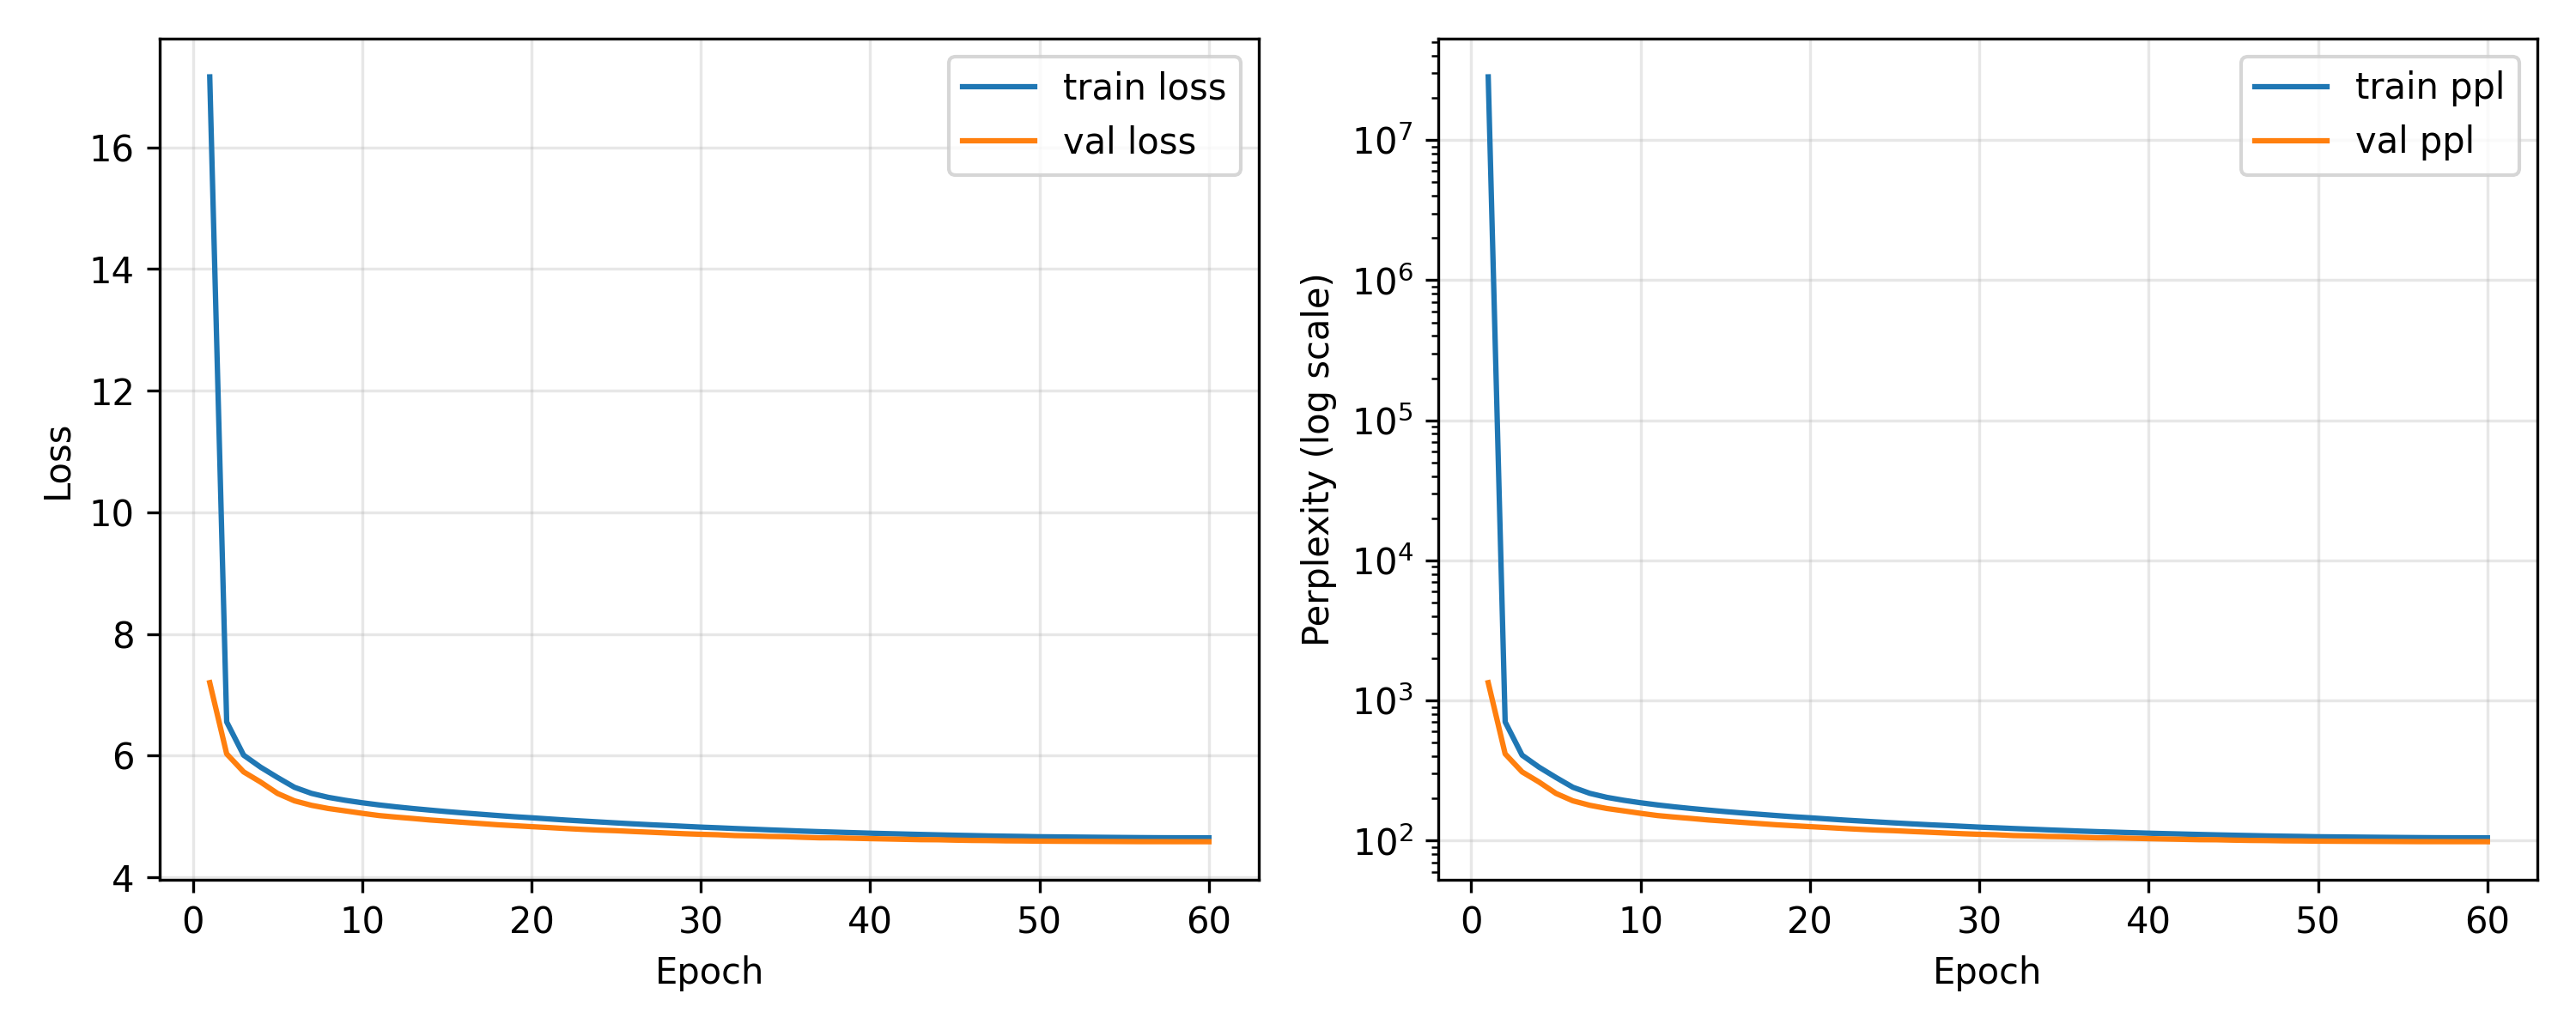
\includegraphics[width=0.96\linewidth]{../Figure/loss_ppl_curves.png}
		\caption{训练集与验证集loss、perplexity变化曲线}
	\end{figure}

	从图1可以看到，loss在前几轮下降最快，之后进入较慢的收敛阶段。右侧困惑度曲线使用对数纵轴，以避免第1轮极大的训练困惑度压缩后续变化。模型最开始几乎无法给出稳定预测，随后快速学习到唐诗语料中的高频字、常见词组和标点模式；训练后半段困惑度仍在缓慢下降，但改善幅度明显变小。这说明模型已经学到基本语言模式，但由于任务本身是开放式文本生成，同一上下文后可能存在大量合理后继字符，因此困惑度不会像分类任务中的loss那样下降到很低。

	\begin{figure}[H]
		\centering
		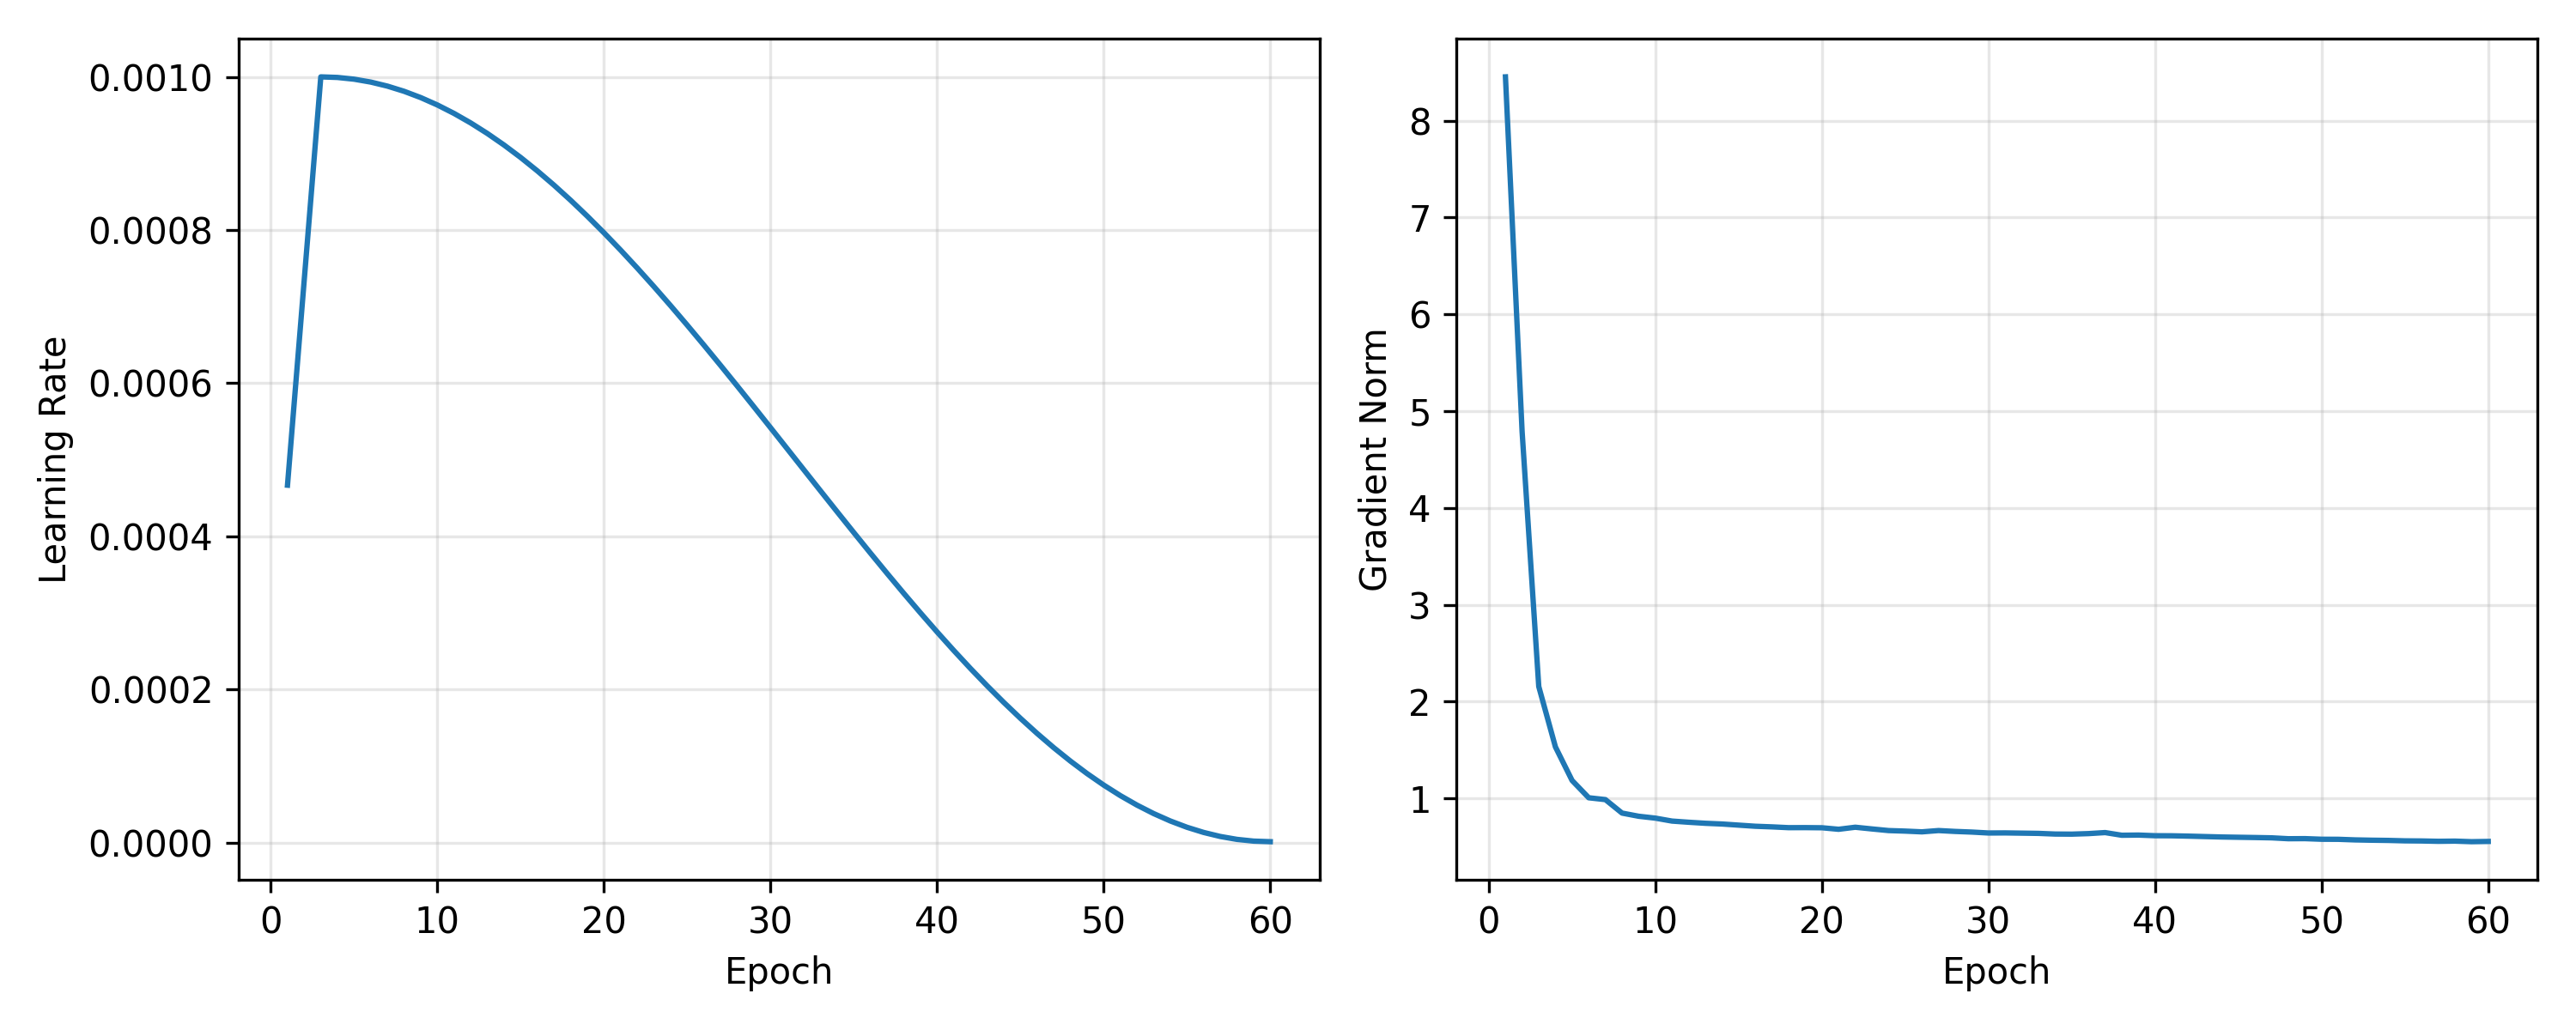
\includegraphics[width=0.96\linewidth]{../Figure/lr_grad_curves.png}
		\caption{学习率与梯度范数变化曲线}
	\end{figure}

	图2展示了学习率和梯度范数的变化。前3轮学习率逐步升高，帮助模型从随机初始化平稳进入训练；之后余弦退火逐渐降低学习率，使后期更新幅度减小。梯度范数在第1轮较大，随后快速下降并稳定在较小范围，说明梯度裁剪和学习率调度能够较好地控制RNN训练中的不稳定问题。

	\section{普通诗句生成}
	普通续写代码先将给定首句拆成字符列表，使用\texttt{<START>}初始化模型状态。生成前若干步时，不直接采样，而是强制将首句中的字符依次喂入模型，使隐藏状态吸收给定首句的信息；首句结束后，再根据模型输出logits进行top-p采样。相比直接取概率最大的字符，top-p采样保留了一定随机性，可以避免生成结果过于单调。

	\begin{lstlisting}
def generate(model, start_words, ix2word, word2ix, device,
             max_len=MAX_GEN_LEN, temperature=TEMPERATURE, top_p=TOP_P):
    results = list(start_words)
    input_tensor = torch.tensor([word2ix["<START>"]]).view(1, 1).to(device)
    hidden = None

    with torch.no_grad():
        for i in range(max_len):
            output, hidden = model(input_tensor, hidden)
            if i < len(start_words):
                w = results[i]
                next_idx = word2ix.get(w, word2ix["<START>"])
            else:
                logits = output.data[0]
                sorted_logits, sorted_indices = torch.sort(logits, descending=True)
                sorted_probs = torch.softmax(sorted_logits / temperature, dim=-1)
                cumsum = torch.cumsum(sorted_probs, dim=-1)
                keep = cumsum <= top_p
                keep[0] = True
                filtered_probs = sorted_probs * keep.float()
                filtered_probs /= filtered_probs.sum()
                chosen = torch.multinomial(filtered_probs, num_samples=1).item()
                next_idx = sorted_indices[chosen].item()
                w = ix2word.get(next_idx, "<EOP>")
                results.append(w)
            input_tensor = input_tensor.data.new([next_idx]).view(1, 1)
    return "".join(results)
	\end{lstlisting}

	以下为实际运行模型得到的普通续写结果：

	\poembox{首句：湖光秋月两相和}{
	湖光秋月两相和，落日江南一半愁。
	}

	\poembox{首句：白日依山尽}{
	白日依山尽，青山万里平。天寒云外出，水阔楚山低。流水逢归客，春风入竹林。明朝更惆怅，更寄旧时人。
	}

	\poembox{首句：海上生明月}{
	海上生明月，还应忆九天。春风开露叶，玉树含芳菲。今日湖中月，同来旧思君。
	}

	这些输出在局部词组和句法上已经具有明显的唐诗风格，例如“落日江南”“青山万里”“春风开露叶”等短语比较自然。但模型仍然存在开放式生成中的常见问题：一是整首诗主题不一定始终集中，二是长距离语义递进较弱，三是有时会把较常见的意象反复组合。其根本原因在于模型只通过字符级语言建模学习局部上下文概率，没有显式建模诗歌主题、平仄和对仗结构。

	\section{藏头诗生成}
	藏头诗生成和普通续写的目标不同。普通续写只要求给定首句后继续生成，而藏头诗要求每一句的第一个字严格等于指定藏头字，同时还要保持五言或七言的固定句长。如果直接沿用普通生成策略，模型可能在一句中间提前生成标点，也可能生成长度不稳定的句子，导致五言、七言格式被破坏。因此我将藏头诗实现为一个单独脚本，在生成策略上加入格式约束。

	具体做法是：先用\texttt{<START>}初始化隐藏状态；对藏头字符串中的每个字，强制把它作为当前句第一个字喂给模型；随后采样生成剩余\texttt{line\_len-1}个字，其中\texttt{line\_len}可以设置为5或7；一句内部屏蔽\texttt{<START>}、\texttt{<EOP>}、\texttt{</s>}以及逗号、句号，防止模型提前结束或在句内输出标点；句末再由程序按照位置手动补上逗号或句号。整首诗生成过程中不重置hidden state，使上下句之间仍保留一定上下文连续性。

	\begin{lstlisting}
def generate_acrostic(model, heads, ix2word, word2ix, device,
                      line_len=LINE_LEN, temperature=TEMPERATURE, top_p=TOP_P):
    model.eval()
    for word in heads:
        if word not in word2ix:
            raise ValueError(f"'{word}' not in vocabulary")

    poems = []
    hidden = None
    with torch.no_grad():
        _, hidden = feed_word(model, word2ix["<START>"], hidden, device)

        for i, head in enumerate(heads):
            line = [head]
            output, hidden = feed_word(model, word2ix[head], hidden, device)

            for _ in range(line_len - 1):
                next_idx, word = sample_word(output, ix2word, word2ix)
                line.append(word)
                output, hidden = feed_word(model, next_idx, hidden, device)

            punctuation = "。" if i % 2 == 1 or i == len(heads) - 1 else "，"
            line.append(punctuation)
            if punctuation in word2ix:
                _, hidden = feed_word(model, word2ix[punctuation], hidden, device)
            poems.append("".join(line))
    return "\n".join(poems)
	\end{lstlisting}

	下面给出实际运行得到的藏头诗结果。可以看到，在固定句长和句内标点屏蔽后，每句首字和句式都比较稳定。

	\poembox{五言藏头：深度学习}{
	深山幽径可，\\
	度地隔溪深。\\
	学院时时见，\\
	习门声渐闻。
	}

	\poembox{七言藏头：丰川祥子}{
	丰年今日在京都，\\
	川路何妨在白云。\\
	祥水自从名不见，\\
	子孙难见好相过。
	}

	\poembox{七言藏头：千早爱音}{
	千里云山万里愁，\\
	早秋城郭旧时秋。\\
	爱君何事君为乐，\\
	音信谁知此意稀。
	}

	\poembox{五言藏头：长崎素世}{
	长安风雨老，\\
	崎岖傍空岑。\\
	素彩含长缨，\\
	世上还可怜。
	}

	从输出结果看，藏头约束能够稳定控制每句首字，五言和七言句长也能由\texttt{line\_len}直接控制。相比普通续写，这里的生成自由度更低，但格式更可靠。需要注意的是，强行指定首字也会带来副作用：如果藏头字之间语义关联较弱，模型只能在局部范围内补全每一句，整首诗的主题连贯性可能不如自然生成。如果要实现更强的效果，可以考虑在藏头诗中加入主题词或韵脚约束，使格式控制和语义控制同时发挥作用，但在本实验就不过度展开了。

	\section{总结}
	本次实验基于PyTorch实现了一个字符级自动写诗模型，完成了数据预处理、Embedding-LSTM语言模型构建、训练日志记录、普通诗句续写和藏头诗生成等流程。模型使用两层LSTM建模字符上下文，在输出前加入LayerNorm稳定隐藏状态，并采用weight tying共享输入Embedding和输出投影权重。训练60个epoch后，验证困惑度下降到98.17，模型能够生成具有一定唐诗风格的句子。

	从实验结果看，模型已经能够学习到常见诗歌意象、基本句法和标点节奏，但仍然缺少对全局主题、对仗、格律和平仄的显式控制。普通续写更自然，但句长和结构不完全可控；藏头诗通过固定五言或七言句长、屏蔽句内标点并手动补标点，使输出格式更加稳定。后续如果继续改进，可以尝试引入更强的序列模型、预训练语言模型，也可以在解码阶段加入重复惩罚、韵脚约束，以进一步提升生成诗句的质量。

\end{document}
